%%%%%%%%%%%%%%%%%%%%%%%%%%%%%%%%%%%%%%%%%
% Laboratory Report LaTeX Template
%
% This template has been downloaded from:
% http://www.latextemplates.com
%
% Original header:
%
% This is a LaTeX version of the sample laboratory report
% from Virginia Tech's copyrighted 08-09 CHEM 1045/1046 lab manual.
% Reproduction of this one appendix section for academic purposes
% should fall under fair use.
%
%%%%%%%%%%%%%%%%%%%%%%%%%%%%%%%%%%%%%%%%%

%----------------------------------------------------------------------------------------
%	DOCUMENT CONFIGURATIONS
%----------------------------------------------------------------------------------------


\documentclass{article}

    \usepackage[a4paper,vmargin={30mm,30mm},hmargin={20mm,20mm}]{geometry}
	\usepackage{natbib}
	\usepackage{graphicx}


\title{Location-aware Real Time Strategy Games \\ Master Thesis \\
Winter Semester 2012 - Summer Semester 2013}
% Title

\author{Vadim Costache} % Author name

\begin{document}

\maketitle % Insert the title, author and date

\setlength\parindent{0pt} % Removes all indentation from paragraphs

\renewcommand{\labelenumi}{\alph{enumi}.} % Make numbering in the enumerate environment by letter rather than number (e.g. section 6)

\newcommand{\superscript}[1]{\ensuremath{^{\textrm{#1}}}}
\newcommand{\subscript}[1]{\ensuremath{_{\textrm{#1}}}}



%----------------------------------------------------------------------------------------
%	TABLE OF CONTENTS
%----------------------------------------------------------------------------------------
   
\begin{verbatim}



\end{verbatim}
     
\tableofcontents

\newpage


\section{Introduction: Real Time Strategy games}

The purpose of this paper is to describe the development of a new type of
GPS-enabled mobile game, a Real Time Strategy / Shooter hybrid. The motivation
for this came up during the search for GPS-enabled multiplayer game concepts.

Ever since the first operating system for handheld devices, the spreading of
smartphones has intensifed every year.In 2012, the number of smartphones in the
world has reached one billion, according to Bloomberg\cite{bloomberg} \newline

The rapid expansion of mobile computing presents new challenges and
opportunities for both the user and the developer. The ease of use and the
presence of touchscreens, GPS receivers, gyroscopes, accelerometers and, since
recently, even barometers gives way to new approaches in developing
games.\newline

In this paper, we will define a number of computer game genres, classify some of
the most popular location-aware games and game platforms and present the
evolution of the concept and development of a game type prototype. This game of
a genre that has a long legacy among computer games, but is not yet known to the
location-aware mobile context. The new genre is that of `Real Time
Strategy`(RTS)\cite{rts} games. We will do that with a subgenre
of RTS, called Real Time Tactics(RTT)\cite{rttvsrts}. For reasons that will be
presented throughout this paper, the type of game can be considered an
RTT / Shooter hybrid. \newline

\subsection{What is Real Time Strategy?}

RTS games are defined as real-time (continuous time) competitive games, in which
several players fight against each other, either in a skirmish or team versus
team. The purpose is to defeat the opponents by taking real-time decisions on
managing resources and troops. The focus is, therefore, on three key elements:
\textbf{managing resource gathering}, \textbf{building a base to provide troops}
and \textbf{battle tactics}.\cite{rts}\newline

This project will focus on a subgenre of RTS, Real Time Tactics(RTT) - which,
instead of managing all three aspects of RTS, focuses on \textbf{battle
tactics}.\newline

Because it is essentially a simplified approach to RTS\cite{rttvsrts}, RTT can
provide a good proof of concept and at the same time simple and enjoyable
playability. The advantage of having a RTT GPS-enabled game versus RTS is that
it greatly reduces the play time, requires less skills and has the potential of
being less stressful than RTS.\newline

\subsection{Real Time Strateg versus Turn Based Strategy}

Turn Based Strategy games\cite{rtsvstbs}(such as chess and board
games, for example) allow the player to take his time and plan every move.
Implicitly, the duration of the game is greater. This type of game is not in the
scope of this project, yet it deserves mentioning, as there are many such games
for mobile devices. Some notable implementations are the ones of Scotland
Yard(Ravensburger GMBH), Catan(Catan GMBH) and Monopoly(Hasbro, Inc.).\newline

In particular, there are two implementations for Scotland Yard upon which a
comparison has been made on whether it is better to port a board game in a
real-time(continuous-time) or turn-based mobile GPS-based game\cite{rttvsrts2}.
These two implementations are Mobilis XHunt(turn based) and MisterX
Mobile(real-time). The comparison has been made on 10 aspects: Fun, Smooth
Progression, Dynamic Gameplay, Ease of play, Stressless Gameplay, Communication,
Strategy, Clear Rules, Low Risk, Education. The conclusion was that there was no
favorite between the two, but it has been concluded that these 10 aspects have
different weights for the player and that Fun, Smooth Progression and Dynamic
Gameplay have a higher individual weight to players than the
rest.\cite[p. 5]{rttvsrts2}\newline

Based on the knowledge gathered from the above-mentioned comparison, the aim of
this project will be to maximize the interactivity and dynamics of the RTS game.


\section{Location-Based Augmented Reality Games}

Ever since the first operating system for handheld devices, the spreading of
smartphones has intensified every year.\newline

The rapid expansion of mobile computing presents new challenges and
opportunities for both the user and the developer. The ease of use and the
presence of touchscreens, GPS receivers, gyroscopes, accelerometers and, since
recently, even barometers gives way to new approaches in developing
games.\newline

Although it is one of the oldest additions to the smartphone, the GPS-enabled
smartphone is still not ubiquitous. As of now, each company's flagship
and most of their mid-level smartphones are GPS-enabled. This makes way to the
propagation of GPS gaming. Although the concept is old, very few attempts have
been made in this direction and this branch of game development may be
considered to still be in one of its early stages of maturity.\newline

This paper is a proposal for extending the genre of mobile real-time multiplayer
location-based games.

\subsection{Location-based games}
Location-based games take advantage of the mobile devices' built-in receivers
for global positioning. They provide the user's location with an accuracy
ranging from a few to a couple dozen meters. Because the most mobile devices in
the world today rely on the Global Positioning System(only recently support for
GLONASS has been added to smartphones), we can use the term GPS-games.\newline

GPS-games came up long before this feature has become ubiquitous in mobile
phones and tablets. One of the first widespread GPS-games is Geocaching. It is
composed of two parts: 
\begin{enumerate}
  \item Placing physical caches at various locations that can be considered
  interesting or worth visiting and publishing their GPS positions (eg. on
  websites).
  \item Searching for various caches by using a GPS device.
\end{enumerate}

Along with the evolution of smartphones came that of the mobile games. GPS games
come in a lot of flavors, from GPS-based tours, adventure and investigation
games to various race games - single and multi player and massively multiplayer
online games.


\subsection{Types of GPS-based games }

There is a number of GPS-enabled games and game authoring tools that are
available for iOS and Android devices. The ones studied for this paper are :
ARIS, Tourality, Wherigo, conTAGion, Shadow Cities, SCVNGR, Please Stay Calm,
Parallel Mafia, Parallel Kingdom, Tripventure, Warfinger, Totem, Portal Hunt,
aMazing, Ingress, MobileWar, Mister X Mobile, Mobilis XHunt, Own This World,
MapAttack.\newline

For better understanding the classification done below, we will first define
each type of game:

\begin{enumerate}
  \item \textbf{Adventure/Investigation Game} - Game in which the player plays
  the role of a character in a story. The primordial characteristics of this
  genre is that it is focused on immersion in the story, puzzle solving and
  investigation, rather than on physical skills. Also, the tendency of this
  genre is towards single player experience, though occasionally multiplayer is
  also implemented (eg. the ARIS-based game 'Mentira').
  
  \item \textbf{Massively Multiplayer Online Game} - This type of game is
  designed to support large numbers of players (even in the number of millions
  in some cases) that play and interact in a persistent virtual world. This type
  of game allows both cooperative and competitive gameplay and is exclusively
  based on multiplayer. Subgenres include MMO Role Playing Games and
  MMO Shooters.
  
  \item \textbf{Casual Game} - Analogous to the MMO, the Casual Game is targeted
  at mass at a mass audience and can incorporate any type of game type. The
  particularity of this genre is that it aims at having simple rules, simple
  gameplay and requiring no specialized skills. 
  
  \item \textbf{Racing Game} - It's a genre defining a broad range of games. In
  the case of computer games, it describes mostly motorized vehicle racing. In
  the mobile context, it mostly describes racing on foot against time or through
  a number of checkpoints.
  
  \item \textbf{Shooter Game} - This one's a subgenre of action games. It
  focuses on first or third person experience, speed, aiming and reaction time.
  Usually the weapon is ranged, although close-combat weapons are included in
  most games.
  
\end{enumerate}

We will now classify the games/platforms based on the genres they best fall in:

\begin{enumerate}
  \item \textbf{Adventure/Investigation Games}
  		\begin{enumerate}
  	  		\item ARIS
  	  		\item Wherigo
  	  		\item Tripventure
  	  		\item Tidy City	  
  		\end{enumerate}
  		
  \item \textbf{Massively Multiplayer Online Games}
  		\begin{enumerate}
  	  		\item Shadow Cities
  	  		\item Please Stay Calm
  	  		\item conTAGion
  	  		\item Parallel Mafia
  	  		\item Parallel Kingdom
  	  		\item Portal Hunt
  	  		\item Ingress
  		\end{enumerate}
  		
  \item \textbf{Casual Games}
  		\begin{enumerate}
  	  		\item SCVNGR
  	  		\item Warfinger  	  		
  	  		\item aMazing 	
  	  		\item Own This World
  	  		\item MapAttack	  	  		
  		\end{enumerate}
  		  		  		
  \item \textbf{Racing Games}
  		\begin{enumerate}
  	  		\item Tourality  	  		 	  		  	  		
  		\end{enumerate}
  		
  \item \textbf{Shooter Games}
  		\begin{enumerate}
  	  		\item MobileWar	  		  	  		
  		\end{enumerate}  
\end{enumerate}

A special category is represented by Mister X Mobile and Mobilis XHunt, which
both bring a board game (Scotland Yard) to the mobile environment. While the
former adapts the board game to real-time gameplay(placing it closer to the
'Multiplayer Racing Games', with elements from 'Real Time Strategy Games'), the
latter falls in the definition of 'Turn Based Strategy' games.

\section{Real Time Strategy Games}

This proposal is for the research and development of GPS-enabled Real Time
Strategy games. They are to be augmented reality games for single player or
multiplayer competitive 'free for all'/'skirmish' and 'team versus team'
games. This category of games offers opportunities to also enhance the
experience for all the previously existing types of GPS-enabled mobile games.

For this project, the proposed games are :
\begin{enumerate}	
	\item \textbf{Territory Takeover}
	\item \textbf{The War Game}
\end{enumerate}

1. The \textbf{Territory Takeover} game is a multiplayer, team versus team
competitive game. The players or game author define an area of play, which will
be divided into multiple divisions. Each division will be marked by a 'flag' (a
GPS marker). To capture the area division, a team must capture its flag. The
game ends when all flags have been captured and the winner is the team with most
captured flags. Each flag may be given a time that a player must spend next to
it in order to capture it. Once a flag (and implicitly the territory) is
captured, it remains so until the end of the game. The winner can be decided on
flag counting or, alternatively, each flag may receive a number of points,
according to the size of the territory marked by it and the difficulty of the
terrain. \newline

This game can be enhanced with the use of virtual tools or weapons. For the
purpose of this project, the following tools/weapons have been considered :
\begin{enumerate}
	
	\item The \textbf{Immobilizer} is an ability that can be used by each player to
	block an opponent from moving. The 'attacker' 'activates' the ability and a
	circle around him is drawn to show the range in which he can shoot. If an
	opponent enters the range area, the 'attacker' will select him on the map and
	shoot. The 'victim' will receive a notification that he is immobilized. A
	circle or rectangle will be defined around him and he will not be allowed to
	move outside of it for a given time, say 30 seconds or 1 minute. If he does, he
	gets disqualified and kicked out of the game. An alternate solution would be
	that the team loses points, for the case that this is the scoring methodology
	implemented.
	 
	\item \textbf{Demobilizer} is an ability that an immobilized player can use.
	For this project, it will only work on the person that uses the ability. The
	effect is that a person that is immobilized gets the waiting time halved.
	
\end{enumerate}
Both the abilities have a common cooldown timer. That means that if a player
immobilizes somebody and is immediately immoblized himself, he won't be able to
use the demobilizer because of the cooldown following the usage of the
immobilizer.

2. The War Game is inspired by Real Time Strategy Games and Airsoft. Two
teams are formed. An area of play is delimited on the map. Each player can
choose between a number of characters. For the purpose of this project, four
characters are proposed: Defender, Marine, Sniper and Heavy Trooper. Each of the
four characters has special abilities and characteristics :
\begin{enumerate}
	
	\item The \textbf{Defender} has the ability to generate shields for short
	periods of time. Members of the team can hide behind those shields for defence.
	The Defender may also act as a Medic and heal or revive members of the team. He
	has low health, long ability cooldowns and a sidearm with short range, small
	damage and fast cooldowns .
	
	\item The \textbf{Marine} has a weapon that can shoot a medium range with
	medium damage and fast cooldowns. He has medium health. 
	
	\item The \textbf{Sniper} has two weapons : the sniper rifle that can shoot at
	distant ranges and deal large damage to single targets and the sidearm, which
	is the same as the Defender's. His health is low, just like the Defender's. The
	sniper shot may penetrate the Defender's shield and cause reduced damage to one
	target.	
	
	\item The \textbf{Heavy Trooper} has three weapons : the bazooka, the sidearm
	and mines. The bazooka is a mid-range weapon with splash damage - it therefore
	can be fired against compact groups, such as the ones that might be hiding
	behind a shield. The bazooka cannot deal damage through the shield, but it may
	be shot next to it, causing damage from the side. The damage to each target
	varies from moderate to small, depending how far they are from the center of
	the 'projectile explosion'. The mines can be placed randomly on the map and
	their 'explosions' will not affect the members of the Heavy Trooper's team.
	Also they cannot be triggered by the members of his team. The damage dealt will
	be moderate, with splash damage, just like the bazooka projectile. The bazooka
	and the mines have long cooldowns, therefore the sidearm is added. The Heavy
	Trooper has high health.
	 
\end{enumerate}

This game has some advantages and drawbacks:\newline
\textbf{Advantages}: It does not require specialized gear and setting, nor does
it need long amounts of time to be played. It can be enjoyed with a bunch of
friends on a sunny weekend afternoon.\newline
\textbf{Drawbacks}: It highly depends on GPS accuracy. This issue may affect
gameplay. It also does not feel as 'real' as real-life games, nor PC
games.\newline


\section{Requirements}

The two above-mentioned games will use a common framework that will enable
multiplayer interaction for both 'free for all'/'skirmish' and 'team versus team'
approaches. They will require a server to centralize player information such as
GPS data and the virtual 'health' attribute. Because the games proposed are
fast-paced, they require quick response times from the server, client and and
the communication protocol between them.

\subsection{Client}
The following technologies have been considered for developing the frontend for
the application : Android, XCode(for Apple iOS) and multiplatoform APIs such as
PhoneGap/Cordova and Titanium. The multiplatform APIs offer the benefit of
the 'code once, deploy everywhere' philosophy, at the cost of
performance\cite{nativevscrossplatform}\cite{nativevscrossplatform2}\cite{nativevscrossplatform3}.
In this case, the approach of using a platform-agnostic framework is
disadvantageous. Therefore, the choice of native app development makes more
sense for this situation.\newline

The client will be developed with Android, due to its accessibility and
versatility and the fact that it's ubiquitous and open source.\newline

\subsection{Server}
The games that are to be implemented will actively rely on communication with a
centralized server. This implies a constant Internet connection on each mobile
device. Also, they require fast, low latency message exchanges. The server
should be able to handle this for players in the numbers of a few
dozens.\newline

The server will be written using NodeJS\cite{nodejs}. NodeJS is a javascript
framework based on the Google V8 Engine that is designed for web server
functionality. Yet, due to the fact that it is a framework and not a standalone
server, one can take advantage of the 'Event Loop' functionality to write
various other types of servers. This particular feat is beneficial to the
purpose of this project. It is also faster than Apache for general purpose, fast
message exchange scenarios\cite{nodejsvsapache}.

\subsection{Communication Protocols}
During a game, active communication must be performed between the mobile devices
and the server in order to multicast all player positions and intentions to all
players. There are two aspects to this approach:

\begin{enumerate}
	\item The game is created on the server, in a so-called `Lobby` which all the
	players join.
	\item The game is created on the server and once the game starts, all players send
	their positions to the server. The server is then responsible to multicasting
	the positions to all the players. 
\end{enumerate}

This is, of course, a subset of the tasks that must be performed by the server.
There will be other information that must be exchanged periodically, such as the
player's health and quantities of various other attributes that will be added
during development and/or proposed during trying out the game. In the general
idea of communication protocol usage, the list of choices has been narrowed down
to three:

\begin{enumerate}
	\item WebRTC - A protocol that is to be part of the HTML 5 standard. It will be
	based on the RTP(Reliable Transport Protocol), which is the base for VoIP
	protocols and is itself based on UDP. It promises to be a very fast standard
	protocol, appropriate for audio and video streaming and massive multiplayer
	games.\cite{webrtc} It is still in draft format and there are no official
	implementations for it. Implementing the protocol itself is outside the scope
	of this project.
	\item WebSockets - A protocol that is part of the HTML 5 standard. It is a low
	latency TCP-based protocol that promisses to replace http in several types of
	web applications.\cite{websockets}
	\item RTP - The protocol on which VoIP and WebRTC are based. It is based on UDP
	and it is designed for real-time streaming of data.\cite{rtp}
\end{enumerate}

From these three protocols, a choice will be made between WebSockets and RTP.
WebRTC is to be left as an option until its official release and implementation
for both NodeJS and Android.

\subsection{Game Elements}

Both games share a number of common features:
\begin{enumerate}
  \item a number of players that are visible on the map
  \item a number of teams, represented by different colors(in the case of
  free-for-all(skirmish) play, the number of teams equals the number of players)  
  \item a number of items that each player can use
  \item item properties, such as range and cooldown times
  \item player health
\end{enumerate} 

The 'War Game' also introduces a number of characters to the game. Each
character type has a different health value and different tools, with specific
properties.\newline

The server must provide a 'game lobby', to which the players connect and prepare
for starting the game. This includes character choice for the 'War Game' and a
'Ready' button. When all players declare themselves to be 'ready', a countdown
starts and then the game begins.\newline

\section{Implementation}

Implementation will mean developing a server and a client application from
scratch, covering all the functionality needed for the games to work according
to the description in section `Real Time Strategy Games`.

\subsection{Schedule}
This project, consisting of one server and one client application, is to be
developed in four steps: 
\begin{enumerate}
  \item \textbf{Development} - During the first iteration of development, the
  most basic features of the game are to be implemented: basic server
  functionality that would allow the game to work, basic client functionality
  and the 'War Game' without all features.(2 months)
  \item \textbf{Testing and Evaluation} - During this phase, the game and its
  functionality will be live-tested for feasibility and quality. New ideas will
  be sought and documented. Most importantly, player feedback will be
  gathered.(1 month)
  \item \textbf{Development} - During the second iteration of development, the
  'War Game' will be completed and, using its framework, the 'Territory
  Takeover' game will be implemented. Bugs will be removed and tweaks will be
  made to the framework and the game concepts to match the player feedback.(2
  months)
  \item \textbf{Evaluation and Completion} -  During the second evaluation
  phase, both games will be tested for playability, player feedback will be
  gathered and the Dissertation Paper will be completed.(1 month)
\end{enumerate}


\subsection{Authoring Tool}
As it is not the focus of this project, the Authoring Tool will comprise the
most basic elements necessary for setting up the game(such as defining obstacles
and probably the border of the gameplay area). Future work might include
modifying and/or adding new character attributes, multiple obstacle types and
probably extending the RTT games to full-fledged RTS.\newline

\section{Documentation on the Games}
Extensive documentation has been found from research done on education-oriented
GPS-games.\cite{pbarg1}\cite{pbarg2}\cite{pbarg3}\cite{pbarg4}\cite{pbarg5}\cite{pbarg6},
describing concepts and approaches in developing platforms and games to this
end\cite{pbarg3}, porting them to different locations\cite{pbarg4}, comparing
them and discussing their functionality\cite{pbarg6}\cite{pbarg1}\cite{pbarg2}
or discussing their effect and usefulness\cite{pbarg1}. Unfortunately for the
direction of this particular project, this documentation focuses exclusively on
GPS-enabled Adventure Games.\newline

The lack of documentation for the other games, except their websites has left
trying them out one by one as the only option to understand their components and
functionality. Additional information was retrieved from video descriptions,
examples and reviews of the games.\newline

During the preparation of this proposal paper no games or documentation have
been found on GPS-enabled Real Time Strategy games. From the searches performed,
no location-aware mobile games have been found to fall in the genre of RTS.
However, one has been found in the genre of `Shooter Games` - MobileWar.\newline

The purpose of this project is to create a framework on which the GPS-enabled
Real Time Strategy games 'Territory Takeover' and 'The War Game' will be
implemented as proof of concept. This framework is to be extended during future
work. The names of the games themselves are chosen only by their descriptive
nature and are prone to change during the steps of development and evaluation.

\section{The project : obstacles and changes}
The two games are proposed with group teambuilding and recreation in mind. Both
games require team strategy and cooperation. Territory Takeover allows for both
team versus team and free for all gameplay, allowing for both small and large
groups to play. The War Game is to be a fast paced game spanning a time interval
in the range of a few tens of minutes. Although it is a RTS Game and not a
Shooter Game, the 'War Game' can be seen as a more casual approach to Airsoft.
Where it lacks the realism of Airsoft or the immersion of classical computer
Real Time Strategy games, it gains in the intensity of real-life experience and
teamwork, without requiring specialized equipment(Airsoft) or highly developed
skills(computer Real Time Strategy games).

%\\\\\\\\\\\\\\  MASTER THESIS HERE\\\\\\\\\\\\\\\\\\\\\\\\\\\\\\\\\\\\\\\\\\\\\\\\\\\\\\\\\\\\\\\\\\\\\\\\\\\\\\\\\\\\\\

\section{The development of the game}

This section will follow the development of the application. The backend,
frontend and mechanics of the game will be analyzed and presented in their
evolution. \newline

The game is composed of three parts : \newline
\begin{enumerate}
  \item \textbf{Mobile App Frontend} - A set of menus for setting up the game
  and a GUI on top of Google Maps for the game itself.
  \item \textbf{Mobile App Backend} - The core of the app. This includes the
  modules for communicating with the server, for in-game protocols and
  mechanics.
  \item \textbf{Server} - All players will communicate with each other through a
  central server that can only host one game at a time.  
\end{enumerate}


\subsection{Initial plan}

The original plan was to develop and Android and iOS app, using a development
framework such as PhoneGap. This would assume Javascript / JQuery programming
for the UI and application backend. The communication was planned to be
established through Websockets. Therefore, for optimum performance, NodeJS was
to be used on the server side. For the location presentation, the Google Maps
API was to be used.

\subsection{Unified vs. Native Frameworks}

Once an idea of how the game should look like was crystalized, I started looking
for unified frameworks for cross-platform mobile development. The first choice
was PhoneGap, which I have used in the Agile Lab in the previous summer and was
a bit familiar. The other frameworks that I considered were Titanium SDK, Sencha
and Corona. The discussion on which one is better can be resumed to the
conclusion that none of them is appropriate for the development of such a game.
And here are the reasons : 
\begin{enumerate}
  \item The game is fast-paced and will require a fast backend as well as a
  frontend that is as fast as possible. The cross-platform frameworks
  essentially interface only some of the native functionality and display the
  app through a webview - requiring Javascript or a Javascript-based framework
  for creating the interfaces. I have tested some these frameworks on top of
  Phonegap, during the Agile Lab. The purpose was then to find the fastest
  solution for static menus and slow-paced UIs. Even then, the outcome has been
  disappointing. Qooxdoo, ExtJs and JQuery were tried out. Qooxdoo
  performs faster than the other two, but makes it very slow and tedious to
  develop a complex UI. Still, it is slow for the purpose and feels nonnative. 
  After reading a few articles that compare Phonegap, Titanium, Sencha and
  Corona, I have concluded that with or without various advantages and
  disadvantages between them, they are all similar in performance - and
  therefore too slow for the development of this game.
  
  \item Being a game prototype, all the details on which features of the phone
  or of the operating system will be used were unclear. I found it unwise to
  develop on a platform that only permits a number of features that are common
  to all platforms.
  
  \item Developing native code can prove to be easier, as for example the
  Android development community is much larger than that of Phonegap developers.
  The support is both more intensive and extensive for native platforms.
  
\end{enumerate}

From this point on, I gave up the unified frameworks and had to decide between
iOS and Android development. This was an easy choice : Android develpment is
free, while iOS development requires a paid developer account and XCode runing
on MacOS exclusively. Therefore, I chose Android. 


\subsection{Communication Protocols}

Initially, I have planned to use Websockets for the client-server communication.
The reasoning behind it has two main arguments : 
\begin{enumerate}
  \item Websockets is an HTML5 protocol currently presented in draft by the
  IETF. This protocol provides reliable two-way communication between a server
  and a client and manages various complex issues or network features that come
  above TCP. This future standard is developed to replace HTTP and add
  functionality for technical aspects that HTTP was not covering. The reason for
  using Websockets for the client-server communication was that it promises to
  abstract a lot of protocol management issues, while offering speeds close to
  plain TCP. Also, for the game to run properly, UDP and its child protocols
  cannot be used - total reliability is required in the communication. 
  
  \item Websockets communication can be implemented in NodeJS, which is a
  framework well suited for fast-paced message exchanges and which has been
  proven more scalable than, for example, Apache Tomcat. 
\end{enumerate}

As I decided to develop the server in NodeJS, the first choice was to use the
Socket.IO Websocket plugin. For the client side, I chose Autobahn for Android.
The only alternative for Autobahn was not free. After developing a basic
Websockets client with Autobahn for Android, I realized that they do not
communicate. After a lot of searching, I found out that the protocol
draft version that Socket.IO is using is different than that used in Autobahn,
and unlike Autobahn, Socket.IO uses an HTTP handshake for establishing the
connection. The Websocket-Node and ws NodeJS libraries for Websocket
communication were tried out afterwards. Neither were compatible with Autobahn
for Android. Then, I have switched to Python and after some technical
difficulties both in the Autobahn libraries for Android and establishing the
communication between client and server, I decided to give up Websockets and
start off with pure TCP. Because writing code in two different languages feels
slower, I have switched to Java.

\subsection{Google Maps API V1}

The first version of the app used Google Maps API V1. I chose it because it has
more extensive developer support. Unfortunately, the Google Maps API and the
Android Support Library cannot work together at the same time, because they need
to subclass different Fragment classes.

\subsubsection{Map Overlays}

The Google Maps V1 API supports the use of Overlay objects to draw on top
ofthe map. Most tutotials found online make use of the so-called
ItemizedOverlay, which enables easy integration of multiple markers. I have
attempted to use this, but here are my conclusions :\newline 
\begin{enumerate}
  \item The ItemizedOverlay uses features that we may call 'magic' - the
  programmer is kept at arm's distance from understanding exactly what they do.
  The ItemizedOverlay object uses an ArrayList for storing the map markers as
  OverlayItem objects. It also needs a function that gives it the size of the
  ArrayList. 
  
  \item Then, by unknown means, the markers are redrawn onDraw. This has
  proven very difficult to work with. For starters, there is no control over the
  draw process. Then, the OverlayItem objects cannot be stored in another data
  structure, such as a HashMap - which I ended up using.
  
  \item Because of its design, the ItemizedOverlay is fast, but useless for the
  purpose of this app. I chose to replace it with a custom Overlay.   
\end{enumerate}

As a replacement for the ItemizedOverlay, I have started to work on how to
create a custom Overlay that would fit my needs. I realized how simple it is to
modify the onDraw() method and control the display of the markers. This has also
allowed me to change their Drawables(icons) dynamically, according to my needs.
I have added functionality to change the Drawable for a selected marker or for
the marker of a dead character. \newline

A real challenge was to add proper onTap() functionality for the custom Overlay.
The advantage of the already-given-up ItemizedOverlay was that it handled marker
touch events. The new, custom overlay had no such thing implemented. What I have
done was to get the pixel resolution of the screen, along with pixel density
data from the system and consider a 0.2 inch radius around the center of the
touch on the screen (this is what I have estimated to be a circle to describe
the tip of an average human adult finger). That 0.2 inch radius in pixels has
been translated in a radius, in meters, on the Google Map. All markers inside
that radius were considered and the closest to the center of the touch was
chosen. This made choosing a marker out of both crowded and loose situations
relatively easy and natural. The tutorial for this will be added as an annex to
the paper.\newline

\subsection{Google Maps API V2}

The use of the Google Maps API V1 ended when I realized that it is not
compatible with the Android backwards compatibility libraries - that enable the
use of Fragments, for example, in Android versions prior to 3.0. The
compatibility libraries require the use of a custom FragmentActivity and custom
Fragment, FragmentManager, FragmentTransaction objects. \newline

The statistics given by Google about the versions of Android in use were
underrepresenting the situation that I faced when trying to test the app. Only
one of my friends and acquaintances had Android 4.1. The rest carried mid-range
phones with Android 2.2 - 2.3. I convinced two friends to let me upgrade their
OS versions to 4.0, even if they were officially unsupported. This was tedious
and risky. Other friends did not accept such a thing. This led me to realize
that it is unfeasible to test the app, when it was supporting Android versions
starting at 3.0. \newline

With this new information in mind, I started the migration to Google Maps API
V2, which, instead of requiring a MapActivity as wrapper, is using MapFragment.
Therefore, I could use both the support library and the Maps V2 API, which is
included in the Google Play Services libraries.\newline

\subsubsection{Maps API V1 vs. V2}

The migration to V2 is very destructive and at first feels quite unnatural. The
entire logic is changed. In V1, the map is rendered through a MapView object
that can be manipulated in a more direct and intuitive manner - lower level
access is both possible and needed. In contrast, the V2 map is accessed through
a GoogleMap object, which is no longer subclassing View. Therefore, it cannot be
manipulated in the same manner. Adding markers is done through the .addMarker()
method of the GoogleMap object. The same applies to drawing circles. Now lists
must be kept for all drawn objects, not for future redrawing, but for being able
to remove or change them. The entire Fragment object, along with a lot of
helper classes had to be rewritten completely. All methods helping out the
onTouch event for the custom Overlay were not necessary anymore. Also many
refresh workarounds were thrown away and in the process, the Activity's
runOnUIThread() method was discovered. 

\subsection{Android development}

I must also add the fact that learning how to program in Android was done while
developing. This was often a trial-and-error process, covered with personal
takes on the tutorials found mostly on StackOverflow.

\section{Organization of the project}

Before there was the project, there was a long search. I initialliy wanted to
continue what was done one semester before, in a lab on agile software
development, where 12 people developed a tour app using Phonegap. I wanted to
add multiplayer functionality to the game, but simply seeing everybody on the
map was to simple. Ideas arose from discussing this with my coordinator. Among
them were ideas for including games and side activities. During the next three
months, I have tried all the mobile games that used a GPS and that I could find
on iOS. Most of them were also ported to Android. In the meantime, I have found
out of the existence of Bluestacks, an Android emulator for Windows. A large
number of games were tried out, but many gave a feeling of involvement and some
gave the impression that they will require too much commitment from the player.



In the proposal for the project, I separated the 6 month time in 4 parts : 
\begin{enumerate}
  \item First phase of development - 2 months
  \item First phase of testing - 1 month
  \item Second phase of development - 2 months
  \item Second phase of testing -1 month  
\end{enumerate}

This interval was also supposed to include the writing of this paper, in between
the lines. This schedule has proven unfeasible - not because of the
length of the development phases, but because of the very short length of the
testing phases. Another big part of the development of this app has been played
by the continuous search for the appropriate technologies and practices for the
project - including my own organizing:
\begin{enumerate}
  \item The exploration phase - Creating a UI test (Android), a server test
  (NodeJS, then Python, then Java), a client test(Android). There have also
  been some short UI tests and discussions along the way. This phase took around
  two-three weeks.
  \item The initial development phase - Creating a functional app with the Maps
  API V1 and writing a full-blown server. This was the longest phase - taking
  around one month and a half.
  \item The first testing phase - It lasted for half a day. Preparations for it
  took another few hours (upgrading the OS on two phones from Android 2.3 to
  4.0).I brought a few friends, installed the app on all their phones and tried
  it out for 1 hour (in multiple attempts, with some crashes). After playing
  the game, the friends and I discussed the usability, mechanics and feeling in
  and out of the game, in a focus group approach. A friend and I took notes,
  while we all discussed various aspects of the app. Also the menus and a
  possible logo were discussed. I gathered so much input from them that only
  their proposals would change the face of the app entirely. Also this is when I
  realized that I must make the app compatible with Android 2.3 for the least
  (almost 50\% of Android users have this version on their phones).
  \item The second development phase - I have worked for another 3 weeks to
  completely construct a new UI according to the requirements from the testing
  phase and the switch from Google Maps API V1 to V2. I have added a crash
  logging and data usage logging system to the app.
  \item The second testing phase lasted one day. I created a Facebook
  event and invited 10 people that brought Android phones. Most of them also had
  3G sim cards. The game was finally field tested and I could get the opinions
  of the people on the UI, the functionality, the speed of the app.
  \item The documentation phase is ongoing. This is the paper documenting the
  development of the app.
  
\end{enumerate}

\subsection{Kanban}

For managing the development steps of the app, I have mainly used a simplified
Kanban board. As is specific to Kanban, I have gradually proposed stories and
fragmented them into tasks, where necessary. As I worked alone, all team aspects
of this organizational system have been removed. The fields that have been kept
are an 'Input Queue', two 'Development' slots, the 'Integration' slots and the
'Live slots'.\newline

There is a significant physical difference between the board that I used, versus
the one used in the 'Agile Lab' from the previous semester. The first used a
whiteboard with slots defined by lines drawn with a marker, on which the stories
and tasks were held with magnets. Although this has been highly efficient for
the short duration of the lab, I don't condsider it useful for an endeavor of
longer duration - stories and tasks and magnets are lost. The markers get
misplaced and paper is often not found. For the development of the app, the
Kanban board was made out of an actual wooden board, on which transparent
plastic envelopes of two different sizes were placed as slots for the stories
and tasks. Also, under the board, three more slots have been added : one for the
papers for the stories and tasks, one for the utensils(markers and pens of
various colors and scissors) and the last one for the finished stories and tasks
that did were pushed outside the board. This gave better control over
the location of everything needed and multiple stories could be placed
in the same slot. For example, the two 'Input Queue' slots have proved
to be not enough for the influx of ideas, and proposals for modification. Also,
the 'Live' slots were not used for single stories, but for groups, as will be
described below. \newline

A personal touch has been added to the Kanban board : the 'Development' slots
have only been used at the very beginning of the project. What I have noticed is
that the developer must have a number of stories and tasks at hand, for
orientation. I have personally lost track of what I was doing when the
'Development' tasks were at the appropriate locations on the board. As a result,
I stopped using the two slots on the board and created a separate slot on the
wall, next to my main monitor. Having all the stories that I was working on has
proven much more useful and straightforward.\newline

I have noticed that many stories are linked in various ways. I was writing the
stories and grouping them according to their connectedness in various aspects -
from similar functionality to work in the same few classes. According to these
criteria, I have treated stories in groups, mentally separating them. For
my future work on this project, I propose adding a few more slots on the wall,
in front of the programmer. In each slot, the programmer can put together
stories with common traits. Also, I recognized the importance of having the full
story in front of you, even if you are working on only one task from it. Having
the big picture at all times is just as important as dealing with the details.
In the case of work within a team, I would have the story and tasks on the
Kanban board, with the names of the developers dealing with each task, while
each developer would have a copy of the story and the tasks from the board
(with the names of the assignees included) in front of his own workstation.
Therefore, a link between the people working at different tasks and between
the tasks themselves would be permanently kept - and synchronization on
overlapping tasks would be easier. Also due to the fact that I treated
stories in bulks of related work, they have been added to the 'Live'
slots based on these same criteria. \newline

As a difference from the Kanban board used in the 'Agile Lab' from the previous
semester, I propose that all completed stories and tasks have their own slot, in
a visible place outside the board. This offers a good morale to all the
developers who see the stack of solved stories thickening. Having a hold
of all the stories also greatly helps write this paper. \newline

\subsection{Unit Testing}

I considered unit testing for this project, but soon gave it up. This
application is a conceptual prototype. A lot of trial and error was done during
development, changes to some piece of functionality occured as often as a few
times a day. I cannot not acknowledge the usefulness of unit testing in a full
blown, large scale project. But in this case, it has proven to be a liability. I
wrote test cases at the beginning, only to find frustration in the fact that the
specifications for the functionality changed very quickly. Also, because this
app has been more of a creative than technical endeavor, I had to keep my mind
more on the ideas than on their implementation. Often, I have started with a
'quick and dirty' approach, tried out how I felt with the implementation, trying
to put myself in the shoes of an unknowing player and only after this organized
and modularized the code.


\section{The game concept}
The app that I developed is temporarily called People With Guns. It is a GPS-
based RTS / Shooter hybrid concept protoype for Android. It can played by
several people (The upper limit has not been established yet. Until now, the
highest number of players in the game is 6.) that choose to join one of two
opposing teams. The purpose of the game is to use 'weapons' and 'powerups' to
defeat the opposing team. By 'defeat', I mean to 'virtually kill' all the
opponents with the available tools. The current 'tools' are as follows :\newline 

The weapons : 
\begin{enumerate}
  \item Pistol
  \item Rifle
  \item Sniper Rifle
  \item Knife   
\end{enumerate}

The 'powerups' :
\begin{enumerate}
  \item Invisiblity Cloak
  \item Shield
  \item Painkillers / Heal
\end{enumerate}

Each item used by a player has the following attributes : 
\begin{enumerate}
  \item Cooldown - The amount of time that has to pass until the weapon can be
  used again.
  \item Duration - The amount of time during which a powerup is in effect 
  \item Damage - The amount of health points that are subtracted upon a hit (or
  added, in the case of the Painkillers) from the target's total available
  health points.
  \item Range - The maximum distance within which a weapon can be fired.
\end{enumerate}

Based on these attributes, we can make a differentiation between weapons and
powerups. Until this point of the game development, weapons have damage and no
duration. The only powerup that also has damage are the Painkillers - they deal
negative damage to the target. The other two powerups, Invisibility Cloak and
Shield, have a greater than zero 'duration' attribute, but no 'damage'.\newline

Some of the attributes of the weapons and powerups will be modified, during a
phase of balancing. I will therefore describe their conceptual construction : 

The weapons : 
\begin{enumerate}
  \item Pistol - Weapon with low damage and medium fire rate. All the character
  types have it. It is the basic and least effective weapon of them all. The
  range is reduced.
  \item Rifle - Weapon with low damage and high fire rate. The damage is higher
  than that of the pistol and the cooldown takes half as long. The range is
  reduced the same as that of the Pistol
  \item Sniper Rifle - High damage weapon with very low fire rate. The range is
  far greater than that of the Rifle and Pistol.
  \item Knife - The weapon that deals the highest damage of all. The cooldown is
  greater than that of the Sniper Rifle and the range is very small. 
  \item Invisiblity Cloak - Powerup that makes the player disappear from the
  map for a short while. While the player is invisible, he cannot be shot.
  The effect duration is short, while the cooldown is lengthy.
  \item Shield - Powerup that reduces the damage taken to half, while it is in
  effect. The duration of this powerup is short and the cooldown is lenghty.
  \item Painkillers / Heal - Powerup that functions like a weapon that deals
  negative damage to the player or his/her friends. It's effective immediately
  and requires a long cooldown time.
\end{enumerate}

For more complexity in the game, a number of so-called 'character types' have
been created, from which players can choose. Thus far, there are four character
types implemented in the game: Marine, Medic, Sniper, Scout. Each of these has a
different number of health points and different weapons. Because the actual
health amount will vary during a phase of character balancing, I will simply
mention the conceptual construction of the characters :
\begin{enumerate}
  \item Marine - Has average health and two weapons: Pistol and Rifle.
  Represents the basic attack unit.
  \item Medic - Support unit with Shield and Painkillers/Heal abilities. Has
  average health. 
  \item Sniper - Attack/ defense unit. Has a Sniper Rilfe for shooting at large
  distances. Has low health.
  \item Scout - Attack unit specialized at sneaking up on the victim. Has the
  'Invisibility Cloak' ability for disappearing from the map and the 'Knife'
  weapon for dealing large amounts of damage within a very small range. Has
  large health.
\end{enumerate}

Another character has been created for testing purposes. It has been called the
'All Encompassing' and posesses all the weapons and skills presently existing in
the game and very large health. This character has inadvertently opened a window
for two more game types: 
\begin{enumerate}
  \item 'David versus Goliath' - This be a game of many players using regular
  character types versus a much smaller number of 'All Encompassing' characters.
  \item 'Duel' - During the many small tests made to this app beyond the public
  ones, a new style of playing this game has emerged: in the absence of a large
  enough number of players, two can play in the 'Duel' mode : both use the 'All
  Encompassing' character type and, instead of running around, attempt to win
  the game by optimizing combinations of weapons and powerups. This game is
  generally played side by side, for at most a few minutes and has proved to be
  entertaining for the ones who tried it out.
\end{enumerate}

\section{Developing the app}

The development of the app has started on the 14th of January 2013. I had an
idea and no Android programming skills. Everything described from now on is a
process of creativity and learning, intertwined together. But before the
development came the idea, which took three months to concoct.\newline

\subsection{The exploration phase}

The project has started as a proposal to add a multiplayer feature to a tour
app. It was hazy and unstructured. The main point was that the tour app was
targeting individual users. But then, what happens when a larger group tours
together? At the current stage of development, the tour app was offering an
individual experience within the group. So I proposed that the group experiences
the tour together, somehow. \newline

Simply adding the functionality to see all the others within the group on the
map was not sufficient - it would just help if someone got lost or went astray.
Otherwise, I concluded that the user experience would not be improved in any
significant way. Then came the idea of adding small games, hidden caches or
quests and so on. The best idea that still had the tour app as a main platform
was to add detours from the main track as bonuses. On those detours, the people
would have to solve various riddles and small puzzles to get points and find out
about hidden historical spots or interesting facs about the places they are
visiting. \newline

At this point, I contoured the following addon to the main app: the players
would have a main tour path and, as they passed by certain waypoints, would be
offered to go through a bonus/extra track within the area that they are
visiting. If enough of them would agree to do this(by an in-app vote, for
example), they would be presented with a new set of waypoints. These waypoints
would belong to a number of categories: normal waypoints, waypoints where they
would have to split, waypoints where they would have to be together and
waypoints where the whole group would have to wait within a virtual circle,
while one delegate(through vote) would find an item or solve a riddle.\newline

I have come up with another scenario, during the research: In the case of the
group waiting and one member being delegated to solve a riddle or find an item,
a means of cooperation can be brought up: When the team votes and chooses the
delegate, he gets a black screen(no map) and the rest of the team can see
the goal on their phones. Through messages or VoIP, they would help the delegate
navigate to the goal. Then, once the goal has been found or reached, the virtual
circle would disappear and the whole team would be free to move. If anyone would
exit the circle at some point, they would receive penalties and eventually get
disconnected from the game.\newline

Gradually, the ideas for multiplayer features went astray from the tour app,
towards multiplayer GPS-based games. I have explored the idea of GPS-based
puzzle / adventure games and encountered ARIS, a platform for creating such
games. Then I discovered Tourality, and WarFinger GPS, which were the main
sources of inspiration for my app and a few other games that didn't make it in
the main concept, but are to be developed within the game as future
work.\newline

There has been a point when I simply tried out all the GPS-based mobile games
that I could find, and evaluated them. At this point, I already had in mind the
goals for this app: It should move the players to an outdoor environment and
have them walk and run as the main activity, while using the game itself for
an improved experience. Hide and seek and Tag were considered as a model of
entertaining game to be played by a group. The games I found and already
enumerated had, in my opinion, one of two major disadvantages:
\begin{enumerate}
  \item Did not engage the users enough: Games such as Parallel Mafia, SCVNGR or
  Please Stay Calm do not motivate the player to move around much. They also
  offer a very dim user experience in areas with few or no players.
  \item Engaged the users too much: Mobile users, even hardcore gamers, do not
  spend too much time playing on the phone. Rather, they would play on consoles
  or computers, for better immersion. No matter how good the game is, it is
  still displayed on a small phone screen(tablets are not considered in this
  paper). Games such as Ingress and Shadow Cities offer a better and more
  immersive story, but are still demanding of the player and request the full
  focus of the phone owner. This I considered to be a major downside, as per my
  gamer experience, when I get out of my home, I prefer to focus on what happens
  around me and only rarely have the time and will to play such a demanding game
  while on the go. 
  \item Did not motivate the players to move enough - Only Tourality does not
  possess this downside, as it its various game modes are specifically designed
  for running.
  \item Are location-dependent - All adventure / puzzle games such as those
  developed with ARIS, most MMOs such as Parallel Mafia do require the player to
  be in certain places in order to progress through the game. This means that
  the player is put in one of two situations : he 1. has to get out of
  one's way in order to make any progress within the game, or 2. has to travel
  to remote locations in order to play the game in the first place. This might
  be interesting for some, but will certainly fail to capture the attention of a
  worker or student during weekdays.
\end{enumerate}

The engaging problem can also be linked to a time problem. Games that are too
engaging also require a lot of time to be played. My personal take on this is
that the amount of time dedicated to the mobile game should be decided by the
player and not by the game.


\subsection{The initial development phase}

The first development phase was mainly one of searching for the right tools to
get the job done and testing their functionality.\newline

The initial idea was to use Websockets for communication, a NodeJS-based server
and, after some evaluation, native Android. The messages exchanged between
server and clients would be in the JSON format. For this, the choices that I
found viable have been Jackson and Google GSON and json-smart. After determining
their speed and ease of use I have chosen Jackson, as besides its speed, it
offers an easy way of serializing and deserializing JSON directly into a
hierarchy of HashMaps - a method which I personally prefer for a testing phase.
Mapping something yet unknown into POJOs would have been a much harder task on
the long run.\newline

Exploring the use of Websockets has proven unfruitful, as there have been dead
ends :
\begin{enumerate}
  \item The only freely available Websocket library for Android at the time of
  research was Autobahn. The Websocket libraries available for NodeJS were
  Socket.IO, Websocket-Node and ws. None of them worked with Autobahn for
  Android. I eventually found a forum post in which one of the developers of
  Autobahn stated the reasons for the incompatibility between Socket.IO and
  Autobahn for Android: First, the protocol implementations were based on
  different draft versions. Second, Socket.IO used an HTTP handshake for the
  connection - and that was not supported by Autobahn. The same issue applied to
  Websocket-Node and ws. A Python implementation of Autobahn has been tried for
  the server, but after a few unfruitful attempts, I decided on Java. In the
  case of Java, Autobahn for Android does not work. I have identified one of
  them: Autobahn subclasses a Handler object that is part of the Android SDK.
  Because of this and the realization that until Websockets receives its final
  version, I cannot fully rely on the protocol. And for the purpose of a
  prototype application where communication should not be overly complicated, I
  chose TCP.
  
  \item Because of the Websocket issue, but also the subjectively perceived slow
  development pace with NodeJS (Libraries are not documented, autocomplete
  mostly does not work and there is no javadoc equivalent), I have decided to
  switch to Java. Python was also attempted in the meantime, but productivity
  was perceived as low for the same reasons as for NodeJS.  
\end{enumerate}

At the end of these attempts, the tools that I decided upon were native Android
clients, Java server and TCP communication in between. What was left to decide
upon was whether I would use JSON or XML. Based on some research and my need for
this app, I chose JSON - it is easier to use and it takes less bytes to transmit
the same data as it would with XML. I was planning to use simple data structures
for the messages that were to be exchanged between server and clients.\newline

JSON was chosen. But now the question remained: which Java libraries for
processing JSON would I use? After some quick browsing, three names came on top:
Jackson, Gson and smart-json. I did some searching for benchmarks and tried out
Jackson and Gson. I chose Jackson.\newline

Now the tools were readily available and I started developing the app. I split
the development in three sub-phases : 
\begin{enumerate}
  \item A game UI that would add some mock players on the map and provide some
  usability insight.
  \item The server
  \item The whole app, based on the initial UI experience.
\end{enumerate}

In developing the initial game UI, I added three buttons(one for generating a
number of markers ('Generate Markers') on the map, one for further use('Check
Info') and one for shooting ('Shoot')) and a spinner, on top of a MapView. The
spinner served as a weapon selector. Once a weapon was selected (on launch, the
first one in the list was automatically pre-selected), its range would be
drawn on the map. I placed the three buttons in three corners of the screen-
bottom-left, bottom-right, top-left. I placed the spinner to the right of the
'Shoot' button. The functionalities added were as followed :

\begin{enumerate}
  \item 'Shoot' button - Mock method to display a Toast message stating if the
  shot was performed or not and the selected weapon.
  
  \item 'Generate Markers' button - Mock method to randomly generate markers on
  the map (for this game's purposes).
  
  \item 'Check Info' button - sporadic functionality to display a Toast message
  with various info on data structures in the back end.
  
  \item Spinner - selecting weapons to 'shoot'. 
\end{enumerate}

I initially developed the server in NodeJS, then switched to Python and
eventually settled with Java.\newline

\subsubsection{The structure of the server}
 
\begin{enumerate}
  
  \item A 'communication' module for dealing with adding and managing
  connections and messaging.
  
  \item A 'messages' module for managing the incoming and outgoing messages for
  each connection.
  
  \item A 'game' module for handling in-game data, such as keeping track of
  connected players, teams and game status. 
  
\end{enumerate}

\subsubsection{The structure of the 'communication' module}

\begin{enumerate}
  
  \item The 'TcpServer' class that starts listening for incoming TCP connections
  on a given port. 
	
  \item A 'ConnectionManager' class that provides static synchronized methods
  for managing adding and removing connections, MessageSender, MessageReceiver
  and connection keepalive heartbeats.
  
\end{enumerate}

\subsubsection{The structure of the 'messages' module}

\begin{enumerate}
  
  \item A 'Messages' class that contains a number of inner classes for
  categorizing the different types of messages.
  
  \item A 'MessageSender' class that deals with sending messages to a single
  client, but can also access all other instances of this class to multicast
  and/or broadcast messages to all the other clients, when needed.
  
  \item A 'MessageReceiver' class that deals with receiving messages from a
  single client
  
  \item A 'HeartbeatListener' class that listens for heartbeats from the
  connected clients and keeps the connections alive or closes them.
  
\end{enumerate}

\subsubsection{The structure of the 'game' module}

\begin{enumerate}
  
  \item A 'Player' class that stores information about the players (eg. name,
  'profession', health points and position).
  
  \item A 'GameManager' class that manages the addition, removal and management
  of players.
  
\end{enumerate}

\subsubsection{The Server}

Once started, the server listens on a port. When a remote client connects, the
server adds an InetAddress instance containing the IP address of the client.
Then, a Player object with some default values is initialized and a random UUID
is generated. The Player object is added in one of the HashMaps for the two
teams - home team or away team - using the UUID as key. A MessageReceiver and a
MessageSender are instantiated. The MessageReceiver, MessageSender, a Date
object containing the moment of the connection and the newly generated UUID and
added to HashMaps with the InetAddress of the client as key. The server sends a
configuration json containing the already connected players, the available
professions and their attributes(title, health, weapons, description), the
available weapons and their attributes(name, range, cooldown, duration,
description and usage policy). From now on, whether a player remains connected
to the server depends on the so-called heartbeats : The client will send
periodic heartbeat messages to the server. The server will update the Date
object for the last moment when a heartbeat was received. If a delay beyond a
threshold comes up, the client is removed from the server.\newline

The server now acts only as a relay - game state is held on the client
side.\newline

Because TCP does not allow multicasts and broadcasts and UDP was purposely
avoided, methods for sending multicasts and broadcasts were conceived as
follows: When a client sends a message that requires multicast/broadcast, the
server accesses all the MessageSender objects, iterates through all of them and
sends the given message to all of them. This applies to location updates, shot
alerts and in-game messages.\newline

Once a number of players (1 or more) have connected to the server, they may send
'Ready' messages to the server, stating that they are prepared to enter the
game. The server will check on receipt on each 'Ready' message if all the
players connected to the server are 'Ready'. If yes, a countdown timer will be
started: A broadcast with the seconds left until the game starts will be sent to
all the players. After the countdown, an 'Enter Game' message is broadcast to
all the clients. Because the server holds the information on the positions of
all the players, a condition and another message have been added: when the
distance between the average positions of all the players in each team is at
least some given distance(eg. 500m) and each team member is at most some other
given distance(50m) from the average position of his/her team, 'Start Game'
message is broadcast to all the clients. This will later be used to enable the
weapons for all the players only when they satisfy these conditions.\newline

There is no direct disconnect message between server and client. Disconnection
is done exclusively based on the heartbeat interval.\newline

\subsubsection{The Client}

The client is an Android application that uses one Activity and multiple
Fragments. It does not use any compatibility libraries(as the Google Maps V1 API
requires a MapActivity and the support library requires a FragmentActivity for
fragment use) - therefore, only Android versions equal or higher to
3.0(Honeycomb) are supported. 

The client uses seven fragments for the UI: 'Main Menu', 'Info and
Tutorials', 'Settings', 'Lobby','Lobby Settings', 'Loading' and 'Game':

\begin{enumerate}
  \item 'Main Menu' : It is the entry point of the the application (it is the
  fragment loaded by the Activity after it is created). It features three
  buttons: 'Start Game', 'Settings' and 'Exit'. By pressing 'Start Game', the
  player attempts to join the game. If the connection is successful, he is
  brought into the 'Lobby'. Pressing 'Settings' leads to the homonymous
  screen.
  
  \item 'Settings' contains two TextViews for changing the default IP
  address and port of the server to which the client can connect.
  
  \item 'Loading' is an intermediary fragment that shows a loading widget for
  the duration of time during which the connection to the server is established
  and the client receives the config json from the server. Once this process is
  done, it automatically switches to the 'Lobby' fragment.
  
  \item 'Lobby' is the main game preparation fragment. It shows the lists of
  players in the two teams(nicknames, professions and 'Ready' status). The
  fragment features four buttons: 'Back', 'Change Info', 'Change Team' and
  'Ready'. If the 'Back' button, the connection to the server is closed and the
  'Main Menu' fragment is brought to the front. The 'Change Info' button brings
  upon the 'Lobby Settings' fragment. By pressing the 'Ready' button, the player
  toggles his/her 'Ready' status and sends a message containing this status to
  the server.
  
  \item 'Lobby Settings' is the fragment in which the player can change his/her
  nickname and 'profession'. A textbox for the name, a spinner and a
  description textbox for the profession and an 'Ok' button are provided. 
  
  \item 'Game' is the most important fragment in this app: it provides the UI
  for gameplay. It features a fullscreen MapView that displays the map and, on
  top of it, the 'Shoot' button and weapon selection Spinner. Two other buttons
  are kept on the screen and given various functionalities, according to the
  testing needs.
   
\end{enumerate}

The app usage would go as follows: The player opens the app and is presented the
'Main Menu' UI. If the GPS is not on, a dialog will appear informing him of
this and offering two choices: `Turn GPS on` or 'Exit'. If 'Turn GPS on' is
chosen, the GPS Settings page will be shown and the player can switch it on.
Once this is done, the player clicks 'Start Game' and, after being shortly shown
the 'Loading' fragment, is introduced to the 'Lobby' screen. Here, one can see
that he has been added to one of the teams(Home Team or Away Team) and has been
given a default nickname('Player') and profession('Marine'). This is where he
chooses a team by clicking the 'Change Team' button or opts navigate to the
'Lobby Settings' screen by clicking the 'Change Info' button and change the
'nickname' or 'profession'. Once the player is ready to play, he will press the
'Ready' button. If all the players that are connected to the server are marked
as 'Ready', the server will send a countdown (which is seen on the client side
through Toasts) followed by a 'Start Game' message - at which point the client
app will automatically introduce the 'Game' UI. All the players are shown on the
map by blue(current player), red(enemies) and green(friends) markers. Above each
marker, one can see the nickname, 'profession' and health points of the player.
The selection of players is done by clicking the markers. A selected player will
have his marker drawn in yellow. Selecting a weapon from the provided Spinner
deselects the currently selected player(if there is any) and draws the weapon's
range around the position of the current player. For using the currently
selected 'weapon' or 'powerup' on one of the players, the current player has to
select the target on the screen and press the 'Shoot' button. If the selection
attempt does not satisfy the 'selection policies' provided by the Weapon object,
the map marker will simply not be selected. Otherwise, it will change color to
yellow. If the target is not within the weapon's range when the 'Shoot' button
is pressed, a Toast message will appear stating the current distance and that
the shot was not performed. Otherwise, a Toast message stating the distance and
damage will be shown and a cooldown countdown will start at the appropriate
entry of the weapon selection Spinner object. Once a player has lost all health
points, a dialog appears saying that the game is over for this player and gives
him the sole option to exit the game in progress and return to the 'Main Menu'
screen. Once a player exits the game in progress, his marker will disappear on
the maps of the other players. There are no start and end conditions
implemented.

\subsection{The first testing phase}

Contrary to the original plans, the first testing phase took only half a day
with another half day of preparations. Prior tests have been done by the
author alone, with two phones.\newline

A few friends(three male and two female) of the author were invited to play the
game. Three of them had Android phones. The other two have used
the two phones that the author had in posession at the time. Unfortunately, most
of them had Android 2.2 and 2.3 installed. The preparations meant convincing
them to volunteer their phones for an OS upgrade. Android 4.0 was
installed.\newline

The tests have been done mostly indoors, as they revealed various bugs in the
server and client software that were not detected when using only two phones
that were physically connected to the development computer via USB
cables. Because six people had five phones, two of them have played
alternatively. Because not all players had 3G connections available, the game
has been played by connecting to the author's WiFi router. The first bug we
noticed was that occasionally the game would disconnect for no apparent reason.
Others have been related to GPS devices in one of the phones not retrieving the
position and crashing the application or concurrency issues improperly treated.
A few temporary quick fixes got the game on track and we managed to play the
game, firstly indoors for a few times and then outside, after the author's WiFi
router has been placed on the outside window sill. This has inadvertently been a
test of the WiFi coverage of an average old 802.11 b/g router - around 50 - 70
meters radius in an open space describing a half-circle around the router. The
author was the first to accidentally run outside the WiFi coverage and get
disconneted. After the playing was finished, the author(with help from one of
the friends) took notes while everybody has expressed their criticism of the
gameplay, UI and game satisfaction. Although the concept itself has been
positively appreciated, the game UI has received a lot of criticism. Also the
random disconnection of the game from the server has caused a lot of frustration
among the test players. A proposal has been made to allow saving the last
player status and position on the server and allow a timeout until the player
would not be allowed to reconnect. A debate led to the conclusion that
enabling such a feature could allow cheating, through the following scenario: A
player would disconnect from the game, get close to other players, reconnect,
shoot and repeat the sequence - thus avoiding damage and causing frustration to
others. \newline



\subsection{The second develpment phase}

The first testing phase has left a lot of 'todos', notes and guidelines for
better adapting the UI and game mechanics to the player's needs. The second
development phase has addressed these needs with a personal touch from the
author and an influence of the switch to a newer version of Maps API.

\subsubsection{The Server}

\subsubsection{The Client}

The client is an Android application that uses one Activity and multiple
Fragments. 

The client uses seven fragments for the UI: 'Main Menu', 'Info and
Tutorials', 'Settings', 'Lobby','Lobby Settings', 'Loading' and 'Game':

\begin{enumerate}
  \item 'Main Menu' : It has been slightly modified: The 'Start Gane' text has
  been changed into 'Connect to Server' - making its functionality more
  obvious. The logo presented in Figure \ref{fig:game_logo} has been added for
  user feedback. The 'Info and Tutorials' button has been added - it leads to
  a new Fragment that presents the idea adn functionality of the game.
  
  \item 'Info and Tutorials' is a fragment with a number of buttons and a
  ScrollView for displaying text and images. Here, the user will find
  instructions for the purpose how use of the app and detailed descriptions of
  the functionality of the 'Lobby' and 'Game' UIs.
  
  \item 'Settings' has not been modified.
  
  \item 'Loading' has not been modified.
  
  \item 'Lobby' : it has been slightly modified to remember the last used
  nickname and 'profession'. Each player in the team lists now shows the ready
  status of that player and a '\[ME\]' indicator has been added to the current
  player so that he can identify himself in the list. Clicking on one's own
  nickname in the list now navigates to the 'Lobby Settings' screen for
  nickname and 'profession' change. Two background images have been tried out on
  this fragment, for user feedback. They are shown in Figure
  \ref{fig:game_background_black} and Figure \ref{fig:game_background_white} 
  
  \item 'Lobby Settings' has not been modified. A background image has been
  tried out as background, for user feedback. See Figure
  \ref{fig:game_background_lobby_settings}
  
  \item 'Game' has been completely modified. Due to changes in the use of the
  Maps API and tester feedback, it has gone through the most changes. At this
  point, the game screen looks as follows: for all the 'weapons' and 'powerups',
  buttons are aligned starting from the bottom left corner of the screen and
  extending them to the right. From the bottom right corner and going up, on the
  vertical axis, three buttons and a TextView exist: the 'Previous Target',
  friend/foe toggle, 'Next Target' buttons and a TextView that shows the
  distance to the next selected player. If no player is selected, the presented
  text will be '0(Self)'. Otherwise, just the distance measurement is shown,
  with no text. In the top right corner, the default 'My Position' button is
  shown - with its specific icon. In the top left corner of the screen, a
  TextView with large text shows the remaining 'health points' of the player.
  Underneath this TextView lays a spinner for sending predefined messages to the
  team. The full functionality of the UI will be presented below.
  
\end{enumerate}

The typical app use scenario goes as follows: The player enters the game and
sees the 'Main Menu'. The app checks if Google Play Services are installed and
if the GPS is turned on. If either of these conditions is not met, a dialog is
presented: the player must choose to install Google Play Services and/or turn on
the GPS or exit the game. Each dialog directs the user to the appropriate Google
Play or Settings page - where the player only has to either click 'Install' or
switch the 'Enable GPS' toggle to 'ON'.\newline

Once there are no more requirements to be met in order to play the game, the
player can click on 'Connect to Server', be briefly presented with the 'Loading'
fragment and then enters the 'Lobby'. There, if the app was started for the
first time, he can see the default nickname 'Player' and the default
'profession' - Marine. If the app was previously used, the player will see the
last nickname and 'profession' used in previous runs. The server distributes the
players according to team sizes, so the player has an equal chance to see
oneself in either the 'Home' or 'Away' team. Then, the player can opt to change
the team by using the 'Change Team' button. Also, the nickname and 'profession'
can be changed by navigating to the 'Lobby Settings' screen. Once the 'Ok'
button is pressed in the 'Lobby Settings' screen, the changes are saved in the
app and sent to the server for broadcasting, and the player is returned
to the 'Lobby' screen.\newline

At the point where all the players have done setting up, they can send the
'Ready' signal. When all the players are ready (for testing purposes, one
player present on the server is enough to start a game), the five second
countdown is received from the server and the player is now facing the 'Game'
screen.\newline

In order to understand what can be done at this point, a detailed description of
the 'Game' UI is necessary: \newline
 
\begin{figure}[ht]
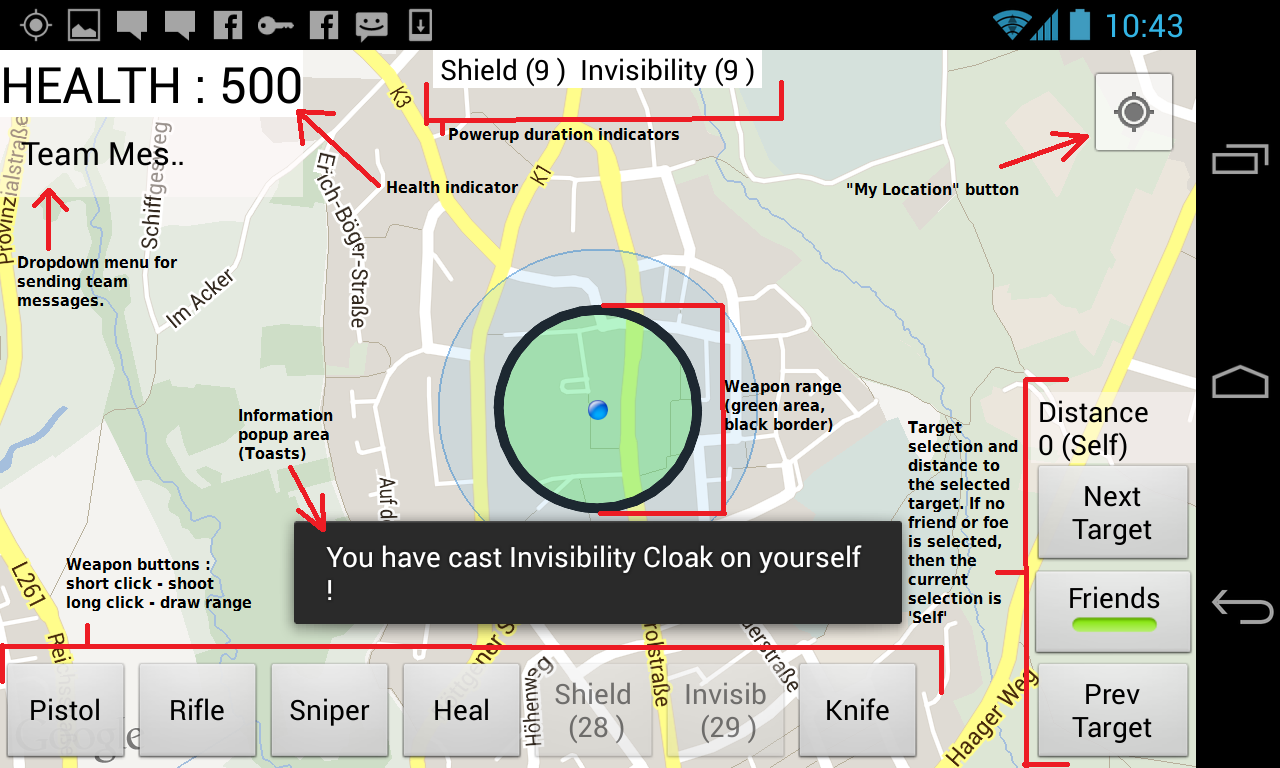
\includegraphics[height=4in,width=7.12in]{./images/android_screenshots/tutorial_game.png}  
\caption{\small \sl The in-game UI \label{fig:game_ui}}
\end{figure}

We can visualize the UI based on the screenshot presented in Figure
\ref{fig:game_ui}. It presents the groups of UI elements on the screen.
We shall now present all of them, separated into groups, by position
(positioning also separates functionality groups, therefore we can also state
that they are presented by related functionality). All the UI elements on the
'Game' UI are programmatically generated - and not from an XML file  :
\begin{enumerate}
  \item \textbf{The bottom of the screen, starting from the bottom-left corner}:
  The 'weapon'/'powerup' buttons are generated once the 'Game' fragment is loaded,
  based on the list of weapons specific to the player's 'profession'. They
  appear from left to right. If less or equal to three weapons are given, the
  buttons will be made slightly larger than otherwise - up to a maximum of six
  (the number of weapons featured in the test 'profession', 'All Encompassing').
  Each button press shoots the 'weapon' or 'powerup', according to a so-called
  'policy' provided in the Weapon object. The policies are as follows: 'self',
  'friends', 'friends and self', 'enemies', 'friends and enemies', 'friends and
  enemies and self'- stating on which kinds of players one given 'weapon' or
  'powerup' can be used. A button long press will draw the range of the
  'weapon'/'powerup' on the map, with the player's position in the center.
  
  \item \textbf{The bottom-right corner of the screen}: The player selection
  buttons and the distance indicator are generated on the vertical axis, starting from the
  bottom-right corner of the screen - in order, the 'previous target',
  friends/enemies toggle, 'next target' buttons, and on top a TextView showing
  the distance to the selected player or '0(Self)' if no player is selected(in
  translation, the 'self' or 'current player' is selected). The friends/enemies
  toggle is used for the obvious reason of quickly choosing between one of the
  two types of players besides the 'self'. The 'next target' button's
  functionality is to find the next closest player from the selected category.
  Let's say that the closest player is already selected. Then, on a press of the
  'next target' button, the second closest player will be selected and so on.
  The reverse applies to the 'previous target' button - which selects the
  previous farthest player if a player is selected and the closest one
  otherwise. The distance indicator serves for the use of an experienced player
  who knows the weapon's distances by heart and does not want to the lengthy
  long click operation to get the weapon's distance shown on the map. The
  players may also be selected by simply tapping their respective markers on the
  map - but through testing it has been determined that in a more intense and
  dynamic situation, selection by clicking on the marker can become difficult
  and inaccurate. Both modes are supported now. One other aspect of player
  selection is the now-vital click in a random unoccupied area on the map for
  deselecting all players(and selecting oneself for, say, self-healing or
  activating powerups on oneself).
  
  \item \textbf{The top-right corner of the screen}: The 'my position' button
  that is provided as an option through the Maps API. Clicking it will cause an
  animation to scroll through the map until the position of the player is
  centered.
  
  \item \textbf{The top-left corner of the screen}: The health indicator is a
  TextView that presents in large text the remaining health points of the
  player. Underneath it lies a spinner with a list of messages that the player
  can send to his/her team. One can do so by clicking on the UI element
  representing the spinner, beneath the health indicator. After the first
  click, the spinner dialog appears and shows the list of messages. The
  player can send one of the messages in the list by clicking it. The dialog is
  canceled by clicking outside it.
  
  \item \textbf{The area in between the two top corners of the screen}: This is
  the area where the powerup duration is dynamically shown during its effect.
  This can be seen when the player casts 'invisibility' or 'shield' on oneself
  or when a friend casts 'shield' on the player
  
  \item \textbf{The area above the weapon buttons}: This is where the
  notifications appear, in the form of Toasts. By default, a toast has a given
  lifespan - but each time a new toast needs to be displayed, it first closes
  the toast currently on display, if it is the case.  
\end{enumerate}

Although they are not yet discretized, thus far we can distinguish three types
of game that can be played with the current setup: the \textbf{default
game}(which requires multiple players, but excludes the 'All Encompassing' game
type), \textbf{duel}(two players choose the 'All Encompassing' profession -
receiving the entire arsenal provided by the game - and try to take each other
out by using various strategies of combining 'weapons' and 'powerups'),
\textbf{David vs. Goliath}(a small number of players choose the 'All
Encompassing' profession and play against a significantly larger number of
players that use all the professions except 'All Encompassing').\newline

Until now, the default game and the duel have been tried out - and they are
fit for different situations: The default game can take up to 20 minutes and is
played across distances varying from small to very large, depending on the mood
and disposition for running of the players. The duel is performed usually by two
players sitting next to each other and takes two-three minutes.\newline

Thus far, no game end condition has been introduced - players who lose all
health points are notified that the game is over for them through a dialog that
gives them two options: quit the game or spectate. The second option implies
that they are marked as 'dead' on the map, cannot be selected and their weapon
buttons are removed from the screen. Still, they can watch the evolution of the
game on their mobile devices. When all players of one team are marked as 'dead'
(they have lost all their 'health points') and at least one player of the other
team still has more than zero health points, it can be considered a win for the
other team. The ending condition has not been implemented, because for this
stage of development of the app it would be just a dialog stating the obvious
'You have won !' message. A more interesting feature may be added in the future,
if imagination or user feedback provides it - or the game may be integrated in a
larger context.\newline

The main functional differences from the first development of the game are:

\begin{enumerate}
  \item A switch from Google Maps API V1 to V2 has been done. This implied
  rewriting the whole UI and several methods in the helper libraries.
  
  \item Because of the switch mentioned above, the custom Overlay object (along
  with the custom tap and marker drawing functionalities), the object
  responsible with position retrieval have been discarded. Position retrieval is
  done through an option provided by the GoogleMap object provided by the Google
  Maps V2 API. The whole marker and weapon range drawing are also done through
  the GoogleMap object - OverlayItem objects have been replaced by Marker
  objects and GeoPoints have been replaced by LatLng instances.
  
  \item The whole UI has been rewritten, having as a result what was described
  above.  
  
\end{enumerate}

Passive disconnection detection functionality has been added in the loop that
waits for incoming messages. The functionality of some weapons and powerups has
been modified. The `Radar` has been removed. The 'Invisibility cloak' and
'Knife' have been added. Powerup duration indicators have been added.\newline

The final message structure in between the server and the client will be
presented in one of the Annexes.\newline

During the second development phase, a lot of decentralization and
modularization of functionality has been done. Classes that only served the
Game UI relying on Maps API V1 have been removed. Others, serving the Maps API
V2 have been added. Various bugs that caused crashes have been corrected. The
starting condition has been reintegrated in the game - it disabled the weapon
buttons until the 'Start Game' message would be received.\newline

\subsubsection{Logging, Testing and Data Usage}
After the first testing phase, the need to log app crashes has come up - as
sometimes it can prove quite difficult to recreate the crash conditions while
solo testing. A logging system based on Logcat capture has been added. Uncaught
exceptions are now caught and logged(they are always the ones crashing the app)
before the app closes. One issue currently not dealt with and considered
benign for the prototype is that the log files(created through classical Java
functionality on the SD Card) can only be seen from the mobile device and not
from a computer communicating with it via USB. This issue was not considered
stringent, as the number of testers and testing devices is still quite low and
manual extraction of crashes is still easier than implementing a solution(The
problem is that these files are signed with a UID and thus cannot be seen by
external devices).\newline

A lot of testing has been done with the 'UI/Application Exerciser Monkey' to
show up potential bugs and crashes. Some bugs have been found and patched - but
one has persisted: Apparently, there are some humanly-impossible combinations of
keyboard and touch inputs that lead to a Spinner dialog crashing the
application. \newline

Another bug that has persisted is that of the WiFi disconnection(3G connections
stay alive). Apparently, this is an Android bug.\newline

As for logging a Logger class has been created, its functionality has been
extended to retrieve the data usage of the app. Because of various compatibility
reasons, the data usage of the entire device during the usage of the app is
retrieved, instead of the usage of the app itself. This means that the data
usage of, say, social network or mail applications adds to the count - but as a
general idea (and not very precise numbers) is needed, it has been considered a
decent solution.

\subsection{The second testing phase}

As the first testing phase, the second one has taken much less time than
initially planned - only one day was necessary. A larger number of friends of
the author were invited. More phones have been brought and almost all had 3G
connection. This time, the app supported Android versions starting with 2.3
- which made it much easier.\newline

A large part of the testing phase has been the preparation: installing the
application on all devices, connecting everyone to the wireless network and VPN
(At the moment of testing, the author lived in a student dorm - and Internet
access was provided through a secure VPN connection. But because everyone's 3G
plan included at most 500MB, Wifi was the first choice). This has proven to be
very frustrating - therefore, everybody switched to 3G and started to play -
firstly indoors and soon after, outdoor. The UI changes have been positively
appreciated by everyone - yet one feature has proven to be quite useless: the
long click on the weapon buttons. The long click draws the range of the weapon
on the map. Our testing scenario, though, has not taken place over large
distances(no one went out of Sniper Rifle range - 150 meters) - therefore the
gameplay has been very fast paced (a game lasted on average between 10-15
minutes) and no-one has actually used the functionality. The distance indicator
has also not been noticed by most. The health indicator, target selection
buttons and shooting functionality of the weapon buttons have been appreciated
as 'right', 'appropriate', 'useful'. A request was made for a finishing
condition and a 'You have won' screen for the winner team - and some sort of
reward system. Another feature that has proven to be more of a liability in this
situation was the starting condition. In the first few games(played indoors),
the players 


\section{Documentation and development}

\subsection{Measurements}


The usage of 'he' should be replaced by 'he/she' and has only been used this way
for the convenience of the author and no other reasons.





\section{Future work}

- switch to Websockets(message exchange) and WebRTC(player position exchange)





\section{ANNEX A - game and game platform websites}



\nocite{teamtags}
\nocite{gps1}



\textbf{ARIS Games}: http://arisgames.org/ \newline

\textbf{Tourality} - http://www.tourality.com/ \newline

\textbf{Wherigo} - http://www.wherigo.com/ \newline

\textbf{conTAGion} - http://www.2clams.com/ \newline

\textbf{Shadow Cities} - http://www.shadowcities.com/ \newline

\textbf{SCVNGR} - http://www.scvngr.com/ \newline

\textbf{Please Stay Calm} - http://pleasestaycalm.com/ \newline

\textbf{Parallel Mafia} - http://www.parallelmafia.com/ \newline

\textbf{Parallel Kingdom} - http://www.parallelkingdom.com/ \newline

\textbf{Tripventure} - http://www.tripventure.net/tripventure/ \newline

\textbf{Warfinger GPS} - http://www.warfingergps.com/ \newline

\textbf{Totem} - http://www.fit.fraunhofer.de/en/fb/cscw/projects/totem.html
\newline

\textbf{Portal Hunt} - http://www.totem-games.org/?q=portalhunt \newline

\textbf{aMazing} - http://www.totem-games.org/?q=aMazing \newline

\textbf{Ingress} - http://www.ingress.com/ \newline

\textbf{Mobile War} - http://www.mobilewar.org/index.php/en/ \newline

\textbf{Mister X Mobile} - http://qeevee.com/projects/misterx \newline

\textbf{Mobilis XHunt} - https://github.com/danielschuster/mobilis/wiki/Mobilis-XHunt
\newline

\textbf{Own This World} - http://www.ownthisworld.com/ \newline

\textbf{MapAttack} - http://mapattack.org/ \newline



\section{ANNEX B - game genre definitions}

% Definitions - Game Genres %

\textbf{Real Time Strategy Game}		
http://encyclopedia2.thefreedictionary.com/Real-time+strategy+game
\begin{quote}
A type of video game in which players exercise strategy along the way, typically
to conquer enemies and reach a final destination without being eradicated. For
example, to win, players decide which routes to take, what needs to be done and
how to do it.
\end{quote}

\textbf{Real Time Tactics Game}
	http://encyclopedia.thefreedictionary.com/Real-time+tactics
\begin{quote}
Real-time tactics or RTT is a subgenre of tactical wargames played in real-time
simulating the considerations and circumstances of operational warfare and
military tactics. It is differentiated from real-time strategy gameplay by the
lack of resource micromanagement and base or unit building, as well as the
greater importance of individual units and a focus on complex battlefield
tactics.
\end{quote}

\textbf{Massively Multiplayer Online Game}		
	http://encyclopedia.thefreedictionary.com/Massively+Multiplayer+Online
\begin{quote}
A massively multiplayer online game (also called MMO) is a multiplayer video
game which is capable of supporting hundreds or thousands of players
simultaneously. By necessity, they are played on the Internet, and feature at
least one persistent world.
\end{quote}
	
\textbf{Adventure Game}		
	http://encyclopedia.thefreedictionary.com/adventure+game
\begin{quote}
An adventure game is a computer-based game in which the player assumes the role
of protagonist in an interactive story driven by exploration and puzzle-solving
instead of physical challenge.[1] The genre's focus on story allows it to draw
heavily from other narrative-based media such as literature and film,
encompassing a wide variety of literary genres. Nearly all adventure games are
designed for a single player, since this emphasis on story and character makes
multi-player design difficult.
\end{quote}

\textbf{Casual Game}		
	http://encyclopedia.thefreedictionary.com/casual+game
\begin{quote}
A casual game is a video game or online game targeted at or used by a mass
audience of casual gamers. Casual games can have any type of gameplay, and fit
in any genre. They are typically distinguished by their simple rules and lack of
commitment required in contrast to more complex hardcore games.[1] They require
no long-term time commitment or special skills to play[\ldots]
\end{quote}

\textbf{Racing Game}
	http://encyclopedia.thefreedictionary.com/Racing+game
\begin{quote}
One of the more common uses of the term racing game is to describe a genre of
computer and video games. Racing games are either in the first or third person
perspective. They may be based on anything from real-world racing leagues to
entirely fantastical settings, and feature any type of land, air, or sea
vehicles. In general, they can be distributed along a spectrum anywhere between
hardcore simulations, and simpler arcade racing games.
\end{quote}
\textbf{Shooter Game}
	http://encyclopedia.thefreedictionary.com/Shooter+game
\begin{quote}
Shooter games are a subgenre of action game, which often test the player's speed
and reaction time. Because shooters make up the majority of action games, it is
a fairly wide subgenre. It includes many subgenres that have the commonality of
focusing "on the actions of the avatar using some sort of weapon. Usually this
weapon is a gun, or some other long-range weapon".A common resource found in
many shooter games is ammunition. Most commonly, the purpose of a shooter
game is to shoot opponents and proceed through missions without dying yourself.
\end{quote}
	
\textbf{Turn Based Strategy Game}
	http://encyclopedia.thefreedictionary.com/Turn+based+strategy
\begin{quote}
A turn-based strategy (TBS) game is a strategy game (usually some type of
wargame, especially a strategic-level wargame) where players take turns when
playing. This is distinguished from real time strategy where all players play
simultaneously.
\end{quote}

\textbf{Location Based Game (Location-enabled Game}
	http://encyclopedia.thefreedictionary.com/location+based+game
\begin{quote}
A location-based game (or location-enabled game) is one in which the game play
somehow evolves and progresses via a player's location. Thus, location-based
games almost always support some kind of localization technology, for example by
using satellite positioning like GPS. "Urban gaming" or "Street Games" are
typically multi-player location-based games played out on city streets and built
up urban environments.
\end{quote}


\section{ANNEX C - Websockets vs. TCP speed}

Websocket is an HTML5 standard aiming at overcoming all the shortcomings of the
already-old HTTP protocol in real-time client-server communication. It is a
TCP-based protocol that uses an HTTP handshake - but that's where the
commonalities stop. The main issue that WS(Websockets) addresses is that with
HTTP, a server cannot send information to the client without being solicited.
Also, WS connections can be kept open and thus bidirectional communication can
be kept alive.\newline

A thorough search for benchmarks for the latency of Websockets versus raw TCP
has returned no result. Instead, several have been found of comparisons between
Websockets and HTTP, Comet and Ajax. Interesting information is found on the
Websocket.org website and reproduced here: \newline





Figure \ref{fig:websocket_frame} shows the size overhead of a Websocket frame
over raw TCP is 2bytes. Figure \ref{fig:websocket_ws_vs_polling} shows the
overhead(in bits per second) of HTTP Polling versus Websockets. We can notice
that in both cases the scale is linear, but the factor is much smaller for
Websockets.\newline

\begin{figure}[ht]
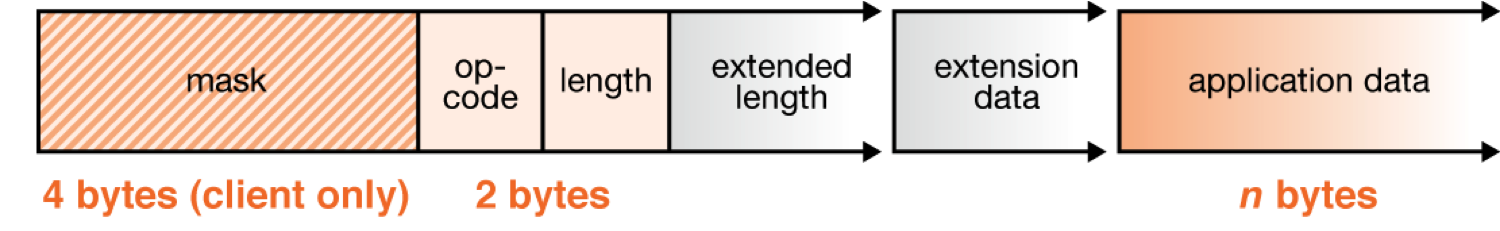
\includegraphics[height=1in,width=7.12in]{./images/websockets/WebSocketFrame.png}  
\caption{\small \sl The Websocket frame \label{fig:websocket_frame}}
\end{figure}

\begin{figure}[ht]
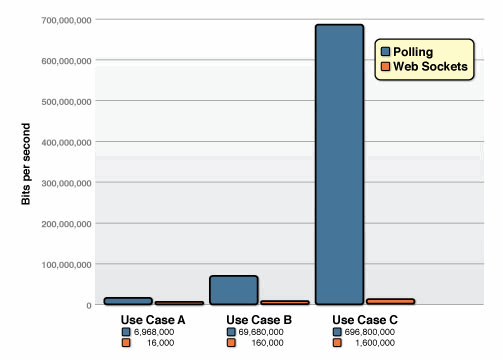
\includegraphics[height=4in,width=7.12in]{./images/websockets/poll-ws-compare.png}  
\caption{\small \sl Websocket vs. HTTP Polling
\label{fig:websocket_ws_vs_polling}}
\end{figure}

After some further searching on the web, a forum answer\cite{websockets3} by the
founder of Tavendo, which develops Autobahn - A well-known set of Websocket libraries for
Javascript, Python and Android:\newline

\begin{quotation}
On a LAN, you can get Round-trip times for messages over WebSocket of 200
microsec (from browser JS to WebSocket server and back), which is similar to raw
ICMP pings. On MAN, it's around 10ms, WAN (over residential ADSL to server in
same country) around 30ms, and so on up to around 120-200ms via 3.5G. The point
is: WebSocket does add virtually no latency to the one you will get anyway,
based on the network.\newline

The wire level overhead of WebSocket (compared to raw TCP) is between 2 octets
(unmasked payload of length < 126 octets) and 14 octets (masked payload of
length > 64k) per message (the former numbers assume the message is not
fragmented into multiple WebSocket frames). Very low.\newline

More so: with a WebSocket implementation capable of streaming processing, you
can (after the initial WebSocket handshake), start a single WebSocket message
and frame in each direction and then send up to 2\^63 octets with no overhead at
all. Essentially this renders WebSocket a fancy prelude for raw TCP. Caveat:
intermediaries may fragment the traffic at their own decision. However, if you
run WSS (that is secure WS = TLS), no intermediaries can interfere, and there
you are: raw TCP, with a HTTP compatible prelude (WS handshake).
\end{quotation}

This answer deems Websockets a fast protocol, appropriate for fast-paced games
such as the one described in this paper.\newline

Moreover, Websockets is designed with security standards and easy development in
mind. It has built - in connection management mechanisms that would easily fit
further development of this application. It would be basically eliminating
potential huge amounts of planning and development overhead induced by starting
a proprietary implementation on top of TCP. \newline


\section{ANNEX D - Node.JS vs. Apache - performance and scaling}

\section{ANNEX E - JSON vs. XML}

\section{ANNEX F - Jackson vs. Gson vs. smart-json}

\section{ANNEX G - Reviews of the games mentioned in the paper}

\section{ANNEX H - Message types and structure in the communication between
Server and Client}

All messages have the following JSON structure: \{messageType: messageNumber,
data: \{\}\}. We are now interested in the data structure. The messageType is a
number that both client and server recognize(as the Messages class is
common).\newline

The Server is active in the message exchange only for the basic administration
purposes: Once a player connects, he receives a configuration json containing
the available 'weapons', 'professions' (with all their attributes) and the list
of already-connected players. It also broadcasts a message telling the existing
players that a new one has connected. When a player disconnects or is
disconnected from the server, a message telling the others that he is
disconnected is sent automatically by the server. Otherwise, the server acts as
a relay.\newline

The Messages class contains a number of inner classes, for proper
classification. We will present the structure, the message types and their
specific JSON structures within:

\begin{enumerate}
  \item \textbf{InGame.ToServer}  
  \begin{enumerate}
    \item CHANGE\_POSITION :
    \{latitude: newLatitude, longitude: newLongitude\}
    
    \item SHOOT :
    \{target: targetUUID, weapon: weaponName, (optional)timestamp: timeStamp\}
        
    \item MESSAGE\_TEAM :
    \{message : messageString\}
      
  \end{enumerate}  
  
  \item \textbf{InGame.FromServer}  
  \begin{enumerate}
    \item CHANGE\_POSITION :
    \{player: playerUUID, latitude: newLatitude, longitude: newLongitude\}
    
    \item SHOOT :
    \{player: playerUUID, target: targetUUID, weapon: weaponName, damage:    
    damageAmount, (optional)timestamp: timeStamp\}
    
    \item MESSAGE\_TEAM :
    \{player: playerUUID, message: newMessage\}
    
    \item GAME\_START :
    \{\} 
        
  \end{enumerate}  
  
  \item \textbf{Lobby.ToServer}
  
  \begin{enumerate}
    
    \item MESSAGE\_ALL :
    \{message: messageString\}
    
	\item CHANGE\_NAME :
	\{name: newName\}
			
	\item CHANGE\_TEAM :
	\{\}		
	
	\item CHANGE\_PROFESSION :
	\{profession: newProfession\}
	
	\item CHOOSE\_WEAPONS :
	this will be made available in further versions where there will be more
	weapons from which to choose
	
	\item READY :
	\{ready : true/false\}    
     
  \end{enumerate}
  
  
  \item \textbf{Lobby.FromServer}
  
  \begin{enumerate}
    	\item ENTER\_GAME :
    	\{\}
		
		\item MESSAGE\_ALL :
		\{player: playerUUID, message: messageString\}
		
		\item CHANGE\_NAME :
		\{player: playerUUID, nickname: newName\}
		
		\item CHANGE\_TEAM :
		\{player: playerUUID, team: newTeam\}
				
		\item CHANGE\_PROFESSION :
		\{player: playerUUID, profession: newProfession\}
		
		\item READY :
		\{player: playerUUID\}
										
		\item PLAYER\_JOINED :
		\{player: playerUUID, name: playerName\}
		
		\item PLAYER\_LEFT :
		\{player: playerUUID\}
			
		\item CONFIGURATION :
		A huge JSON thing that the Server composes based on a Config file and sends it
		to the client. 
		
		\item COUNTDOWN :
		\{secondsLeft: numberOfSecondsLeft\}
		
  \end{enumerate}  
  
\end{enumerate}



\section{ANNEX I - Overlay tutorial}

\section{ANNEX J - Countdown buttons Tutorial}



%----------------------------------------------------------------------------------------
%	BIBLIOGRAPHY
%----------------------------------------------------------------------------------------


\section{Bibliography}
	\bibliographystyle{ieeetr}	
	\bibliography{bibcontent}

\end{document}



